\documentclass[tikz,border=8pt]{standalone}
\usepackage{amsmath}
\usepackage{pgfplots}
\pgfplotsset{compat=1.18}
\usetikzlibrary{arrows.meta,decorations.pathmorphing,positioning}
\definecolor{ink}{HTML}{21352F}
\definecolor{teal}{HTML}{087F7B}
\definecolor{gold}{HTML}{C58B2A}
\definecolor{blue}{HTML}{4B77A8}
\definecolor{rose}{HTML}{B65A62}
\begin{document}
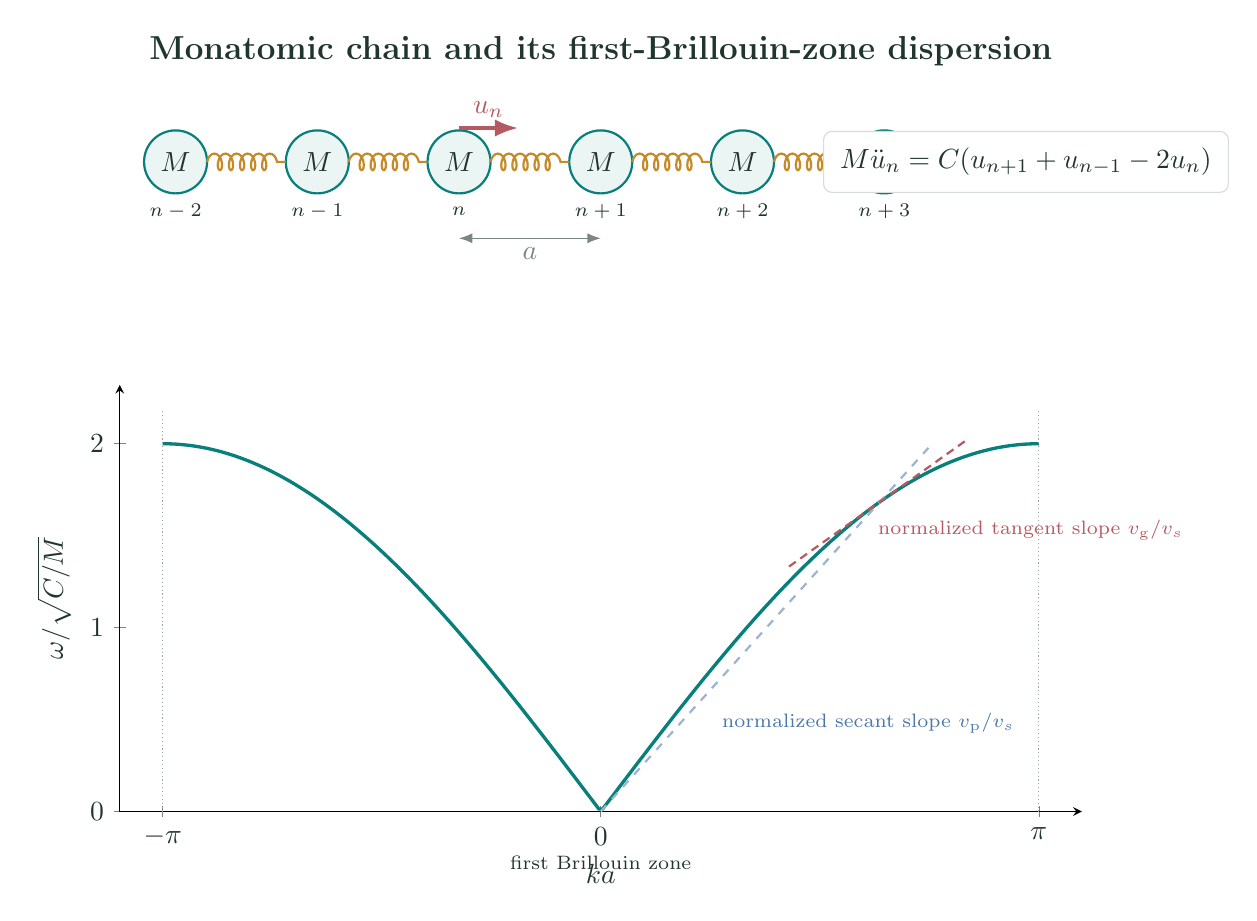
\begin{tikzpicture}[font=\sffamily,text=ink,>=Latex]
  \node[font=\bfseries\large] at (0,4.15) {Monatomic chain and its first-Brillouin-zone dispersion};
  \foreach \x/\lab in {-5.4/$n-2$,-3.6/$n-1$,-1.8/$n$,0/$n+1$,1.8/$n+2$,3.6/$n+3$}{
    \node[draw=teal,thick,fill=teal!8,circle,minimum size=8mm] (m\x) at (\x,2.75) {$M$};
    \node[font=\scriptsize] at (\x,2.12) {\lab};
  }
  \foreach \xa/\xb in {-5.0/-4.0,-3.2/-2.2,-1.4/-0.4,0.4/1.4,2.2/3.2}{
    \draw[decorate,decoration={coil,aspect=.55,segment length=4pt,amplitude=3pt},gold,thick] (\xa,2.75)--(\xb,2.75);
  }
  \draw[<->,ink!60] (-1.8,1.78)--(0,1.78) node[midway,below] {$a$};
  \draw[->,rose,very thick] (-1.8,3.18)--(-1.05,3.18) node[midway,above] {$u_n$};
  \node[draw=ink!18,rounded corners=3pt,fill=white,inner sep=6pt] at (5.4,2.75)
    {$\displaystyle M\ddot u_n=C(u_{n+1}+u_{n-1}-2u_n)$};

  \begin{axis}[
    at={(0cm,-5.5cm)},anchor=south,
    width=13.8cm,height=7.0cm,
    xmin=-3.45,xmax=3.45,ymin=0,ymax=2.32,
    axis lines=left,
    xlabel={$ka$},ylabel={$\omega/\sqrt{C/M}$},
    xtick={-3.14159,0,3.14159},xticklabels={$-\pi$,$0$,$\pi$},
    ytick={0,1,2},
    clip=false]
    \addplot[teal,very thick,domain=-3.14159:3.14159,samples=240]
      {2*abs(sin(deg(x)/2))};
    \addplot[blue!55,dashed,thick,domain=0:2.35,samples=2] {0.841470985*x};
    \addplot[rose,densely dashed,thick,domain=1.35:2.62,samples=2] {0.602337358+0.540302306*x};
    \draw[densely dotted,ink!45] (axis cs:-3.14159,0)--(axis cs:-3.14159,2.18);
    \draw[densely dotted,ink!45] (axis cs:3.14159,0)--(axis cs:3.14159,2.18);
    \node[blue,font=\scriptsize,anchor=west] at (axis cs:.80,.48) {normalized secant slope $v_{\rm p}/v_s$};
    \node[rose,font=\scriptsize,anchor=west] at (axis cs:1.92,1.53) {normalized tangent slope $v_{\rm g}/v_s$};
    \node[font=\scriptsize] at (axis cs:0,-.28) {first Brillouin zone};
  \end{axis}
\end{tikzpicture}
\end{document}
